上节我们从Lamb型方程\eqref{eq:71Lamb}式出发推导了Bernoulli方程的各种变形,如果我们去掉定常流的条件而附加流场无旋的条件,
那么\eqref{eq:71Lamb}式中Lamb矢量为零,由于流体无旋,存在速度势函数$\varphi$,使得$\v{v}=\nabla \varphi$。
积分\eqref{eq:71Lamb}式得到Cauchy-Lagrange 积分方程(CL方程):
\begin{equation}\label{eq:72CLEquation}
\frac{\partial \varphi}{\partial t}+\frac{1}{2} |\nabla \varphi|^2+\mathbb{P}+\Pi=C(t)
\end{equation}

下面是一个应用CL方程的一个例子:

考虑一个长为$2l$的L型两端开口直管,下端封闭,上端与大气接触,里面充满理想均质不可压的液体,如图(\ref{fig:72CL_integral_example}.a)所示:
\begin{figure}[!ht]
 \centering
 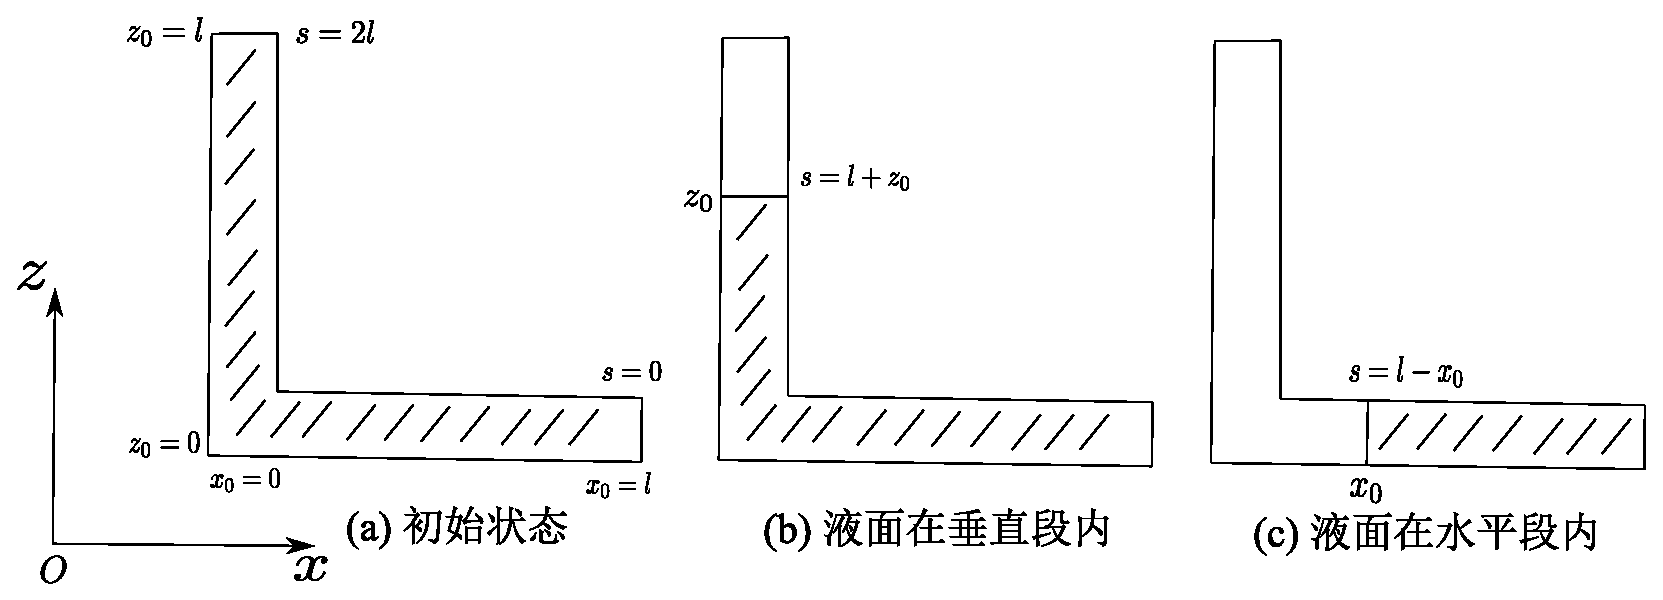
\includegraphics[width=9cm]{CL_integral_example.eps}
 \caption{L型直管}\label{fig:72CL_integral_example}
\end{figure}

当释放直管的下端使液体流出时,
管内压强和出口处的速度会发生突变。我们先来求出口处的速度。为此,取类似于弧长坐标系的一维局部坐标$s$表示离出口处的液柱长度为
$s,0\leq s\leq 2l$,则$\v{v}(t)=-v\v{e_s}$,因为流体不可压,所以$\frac{\partial v}{\partial s}=0$,即$v=v(t)$,又因为速度场有势,
所以存在势函数$\varphi(s,t)$,使得$\frac{\partial \varphi}{\partial s}=-v(t)$,如取$s=0$时速度势为零,则$\varphi(t,s)=-v(t)s$,
所以 \eqref{eq:72CLEquation}式化为:
\begin{equation}\label{eq:72CLEqExample}
-v'(t)s+\frac{1}{2}v^2(t)+\frac{p}{\rho}+\Pi=C(t)
\end{equation}
当直管的下端释放时,分别考虑$s=0$和$s=2l$两端,$p=p_a$,均为大气压,速度均为$0$,$\Pi(2l)=gl$,由上式求出:
\begin{equation}
v'(0)=\frac{1}{2}g,C(0)=\frac{p_a}{\rho}
\end{equation}
如果考虑任意截面$s$处,则有
\begin{equation}
-v'(0)s+\frac{p}{\rho}+\Pi(s)=\frac{p_a}{\rho}
\end{equation}
于是得任意截面$s$处初始时刻压强的分布为:
\begin{equation}
p(s)=p_a+\frac{1}{2}\rho g s-\rho \Pi(s)
\end{equation}
而$\Pi(s)$可写成分段函数的形式:
\begin{equation}
\Pi(s)=\begin{cases}
g(s-l) & l\leq s\leq 2l\\
0 & 0 \leq s < l
\end{cases}
\end{equation}

下面我们考虑液体完全流出时管口的流速,
由CL方程\eqref{eq:72CLEqExample}式得到液面$s=z_0$处和出口处$s=0$时的平衡方程为
\begin{equation}\label{eq:72SimularNewton}
v'(t) (l+z_0)=\Pi(z_0)
\end{equation}
由于$\Pi$是$f$的分段函数,为此,分两阶段考虑:
当液面在垂直段内时,如图(\ref{fig:72CL_integral_example}.b)所示,此时取$z_0$坐标研究问题比较方便:
设$z_0=z_0(t)$,$z_0$随时间减小,$\Pi(z_0)=gz_0,v=-\frac{d z_0}{dt}$,代入到\eqref{eq:72SimularNewton}式中有:
\begin{equation}
-\frac{d^2 z_0}{dt^2} = \frac{g z_0}{l+z_0}
\end{equation}
上式是标准的 Newton 运动学方程,可用能量方法先求出液面降到$f$时液面处速度
$v_{z_0=f}$为:
\begin{equation}
\frac{1}{2}v_{z_0=f}^2=\int_{f}^{l} \frac{g z_0}{l+z_0} dz_0
\end{equation}
解得:
\begin{equation}
\frac{1}{2}v^2_{z_0=f}=g(l-f)+gl\ln \left(\frac{l+f}{2l}\right)
\end{equation}
由此求得$f=0$时的速度为:$v_{z_0=0}=\sqrt{2gl(1-\ln 2)}$
由$v=-\frac{d z_0}{dt}$上式可化为:
\begin{equation}
-\frac{d z_0}{\sqrt{2g(l-z_0)+2gl\ln(l+f)-2gl\ln(2l)}}=dt
\end{equation}
当$z_0$从$l$到$0$时,时间从$0$到液面$z_0$下降到0的时间$T_1$,因此分别对上式两边积分:
\begin{equation}
\int_0^l \frac{d z_0}{\sqrt{2g(l-z_0)+2gl\ln(l+z_0)-2gl\ln(2l)}}=T_1
\end{equation}
变量替换:
\begin{equation}
T_1=\sqrt{\frac{l}{2g}}\int_0^1 \frac{d z_0}{\sqrt{(1-z_0)+\ln(1+z_0)-\ln 2}}=T_1
\end{equation}
数值积分得:$T_1=2.13\sqrt{\frac{l}{g}}$

当液面在水平段内时,如图(\ref{fig:72CL_integral_example}.c)所示,此时由于$\Pi$不随位置变化,由\eqref{eq:72SimularNewton}式可知
速度也不随时间变化。因此液体将以$v_{z_0=0}$的速度匀速流过长为$l$的水平段,用时$T_2=\frac{l}{v_{z_0=0}}=1.28\sqrt{\frac{l}{g}}$
将$T_1$和$T_2$求和即得到液体全部流出的总的时间。

CL积分方程中若速度势$\phi$用动坐标系下的坐标表示,$\nabla$与坐标表示无关,直接改写为$\nabla'$,
但局部导数项$\frac{\partial}{\partial t}$需做相应变换。
考虑到随体导数与坐标表示无关,即
\begin{equation}
\frac{D\varphi}{Dt}=\frac{D'\varphi}{Dt}
\end{equation}
两边展开得
\begin{equation}
\frac{\partial \varphi}{\partial t}+\nabla \phi \cdot \v{v}=\frac{\partial' \varphi}{\partial t}+\nabla' \phi \cdot \v{v'}
\end{equation}
对于$\nabla \varphi$和$\nabla' \varphi$,均表示绝对速度$\v{v}$,只不过一个在绝对坐标系中表示,一个在相对坐标系中。
而$\v{v'}$表示相对速度而不是绝对速度在动坐标系下的表示。

因此我们得到
\begin{align}\notag
\frac{\partial \varphi}{\partial t}=&\frac{\partial' \varphi}{\partial t}+(\v{v'}-\v{v})\cdot \v{v}\\
=&\frac{\partial' \varphi}{\partial t}-\v{v_e}\cdot \v{v}
\end{align}

从而由\eqref{eq:72CLEquation}式得到速度势在相对坐标系下表示的CL积分方程为:
\begin{equation}\label{eq:72CLRelative}
\frac{\partial' \varphi}{\partial t}-\v{v_e}\cdot \nabla'\varphi+\frac{1}{2} |\nabla'\varphi|^2+\mathbb{P}+\Pi=C(t)
\end{equation}

下面是\eqref{eq:72CLRelative}式应用的一个例子:

一半径为$a$的圆球在无限大的理想正压无旋不可压流体中以$\v{v_o}(t)$的速度做变速直线运动,
求流体表面的压力与流体作用在圆球上的合力$\v{F}$。

以$\v{v_o}(t)$的反方向为$z$轴建立空间直角坐标系,则$\v{v_o}=-v_0\v{e_z}$。同时选取固结在圆球圆心的球坐标系作为动坐标系,
在动坐标系中界面边界的法方向为$\v{e_{R'}}$,因此在动坐标系中界面边界方程为:$\v{v'}\cdot \v{e_{R'}}=0$,
换到绝对坐标系中有
\begin{equation}
\v{v}\cdot\v{e_{R'}}=\v{v_o}\cdot \v{e_{R'}}
\end{equation}
参考\cite{Del}中的公式
\begin{equation}\label{eq:72Erxyz}
\v{e_{R'}}=\sin\theta'(\cos\epsilon' \v{e_x}+\sin\epsilon' \v{e_y})+\cos\theta' \v{e_z}
\end{equation}
我们有
\begin{equation}
\v{v}\cdot\v{e_{R'}}=-v_0(t)\cos\theta'
\end{equation}
由于流体无旋,存在速度势函数$\varphi$,使得$\v{v}=\nabla \varphi$,由\eqref{eq:62GradientSphere}式,上式进一步化为:
\begin{equation}\label{eq:72GSBC}
\frac{\partial' \varphi}{\partial R'}_{| R'=a}=-v_0(t)\cos\theta'
\end{equation}
另外,我们还有无穷远的边界条件(速度为零):
\begin{equation}
\nabla'\varphi_{|R=\infty}=\v{0}
\end{equation}
由问题的球对称性,$\varphi$与$\epsilon'$无关,因此上式化为
\begin{equation}\label{eq:72InfityBC}
\frac{\partial' \varphi}{\partial R'}_{| R'\to \infty}=0,\frac{1}{R'}\frac{\partial' \varphi}{\partial \theta'}_{| R'\to \infty}=0
\end{equation}
由于流体不可压,$\varphi$满足Laplace方程:
\begin{equation}
\nabla'^2 \varphi=0
\end{equation}
参考\cite{Del}中的公式,在球坐标系下展开得:
\begin{equation}
\frac{1}{R'^2}\frac{\partial'}{\partial R'}\left(R'^2 \frac{\partial' \varphi}{\partial R'}\right)
+\frac{1}{R'^2\sin\theta'}\frac{\partial'}{\partial \theta'}\left(\sin\theta' \frac{\partial' \varphi}{\partial \theta'}\right)
=0
\end{equation}
我们采用分离变量法求解,对给定的时刻$t$,假设上述方程有形如$\varphi(R',\theta')=f(R')g(\theta')$的解,代入有
\begin{equation}
\frac{\partial'}{\partial R'}\left(R'^2 \frac{\partial' f(R')}{\partial R'}\right)g(\theta')
+\frac{1}{\sin\theta'}\frac{\partial'}{\partial \theta'}\left(\sin\theta' \frac{\partial' g(\theta')}{\partial \theta'}\right)f(R')
=0
\end{equation}
因此
\begin{equation}
\frac{1}{f(R')}\frac{\partial'}{\partial R'}\left(R'^2 \frac{\partial' f(R')}{\partial R'}\right)
=-\frac{1}{\sin\theta' g(\theta')}\frac{\partial'}{\partial \theta'}\left(\sin\theta' \frac{\partial' g(\theta')}{\partial \theta'}\right)
\end{equation}
上式左边与$\theta'$无关,右边与$R'$无关,因此与$R',\theta'$均无关,可令
\begin{equation}\label{eq:72seperationOfVariable}
\begin{cases}
\frac{1}{f(R')}\frac{\partial'}{\partial R'}\left(R'^2 \frac{\partial' f(R')}{\partial R'}\right) =& C(t)\\
\frac{1}{\sin\theta' g(\theta')}\frac{\partial'}{\partial \theta'}\left(\sin\theta' \frac{\partial' g(\theta')}{\partial \theta'}\right)=& -C(t)
\end{cases}
\end{equation}
先考虑\eqref{eq:72seperationOfVariable}的第2式,
考虑到\eqref{eq:72GSBC}式,因此设$g(\theta')=\cos(\theta')$代入上式有$C(t)=2$
再解\eqref{eq:72seperationOfVariable}的第1式
\begin{equation}
R'^2f''(R')+2Rf'(R')-2f(R')=0
\end{equation}
根据Cauchy-Euler方程的解法(\cite{CEEquation}),通过设$f(R')=R'^m$解得$m=1$或$m=-2$,
由无穷远边界条件\eqref{eq:72InfityBC}式只能取
$m=-2$
\begin{equation}
\varphi(R',\theta',t)=A(t)R^{-2}\cos \theta'
\end{equation}
于是\eqref{eq:72InfityBC}式自然满足,代入\eqref{eq:72GSBC}式中求得$A(t)=\frac{1}{2} a^3 v_0(t)$
在动坐标系下,根据上式和求梯度算子的\eqref{eq:62GradientSphere}式,我们有
\begin{equation}
\nabla' \varphi_{|R'=a}=-v_0(t)(\cos\theta' \v{e_{R'}}+\frac{1}{2}\sin\theta' \v{e_{\theta'}})
\end{equation}
于是由\eqref{eq:72CLRelative}式,我们根据在球表面和无穷远处列方程得到:
\begin{equation}
\frac{a}{2}\dot{v}_0(t)\cos\theta'+v_0(t)\v{e_z}\cdot \nabla'\varphi+\frac{1}{2} |\nabla'\varphi|^2+\frac{p}{\rho}=\frac{p_{\infty}}{\rho}
\end{equation}
参考\cite{Del},$\v{e_z}=\cos\theta' \v{e_{R'}}-\sin\theta' \v{e_{\theta'}}$,由上式解出球面压力$p$为
\begin{equation}
p(\theta',t)=p_{\infty}+\frac{1}{2}\rho v_0^2 - \frac{1}{2} \rho \dot{v}_0 a \cos\theta' -\frac{9}{8}v_0^2 \sin^2\theta'
\end{equation}
流体作用在圆球上的合力为:
\begin{equation}
\v{F}=-\oiint\limits_{\Sigma}p\v{n}dA
\end{equation}
这里$\v{n}=\v{e_{R'}}$,是圆球的外法向方向。
结合\eqref{eq:72Erxyz}式我们得到:
\begin{align*}
\v{F}=&-\iint\limits_{\substack{0\leq \theta'\leq \pi\\ 0\leq \epsilon'\leq 2\pi}} p(\sin\theta'(\cos\epsilon' \v{e_x}+\sin\epsilon' \v{e_y})+\cos\theta' \v{e_z})a^2\sin\theta'd\theta'd\epsilon'\\
=&-\v{e_z}\iint\limits_{\substack{0\leq \theta'\leq \pi\\ 0\leq \epsilon'\leq 2\pi}} p a^2\sin\theta'\cos\theta' d\theta'd\epsilon'\\
=& \v{e_z}\iint\limits_{\substack{0\leq \theta'\leq \pi\\ 0\leq \epsilon'\leq 2\pi}} \frac{1}{2} \rho \dot{v}_o a^3\sin\theta'\cos^2\theta' d\theta'd\epsilon',\sin^3\theta'\cos\theta'\text{ 关于$\frac{\pi}{2}$对称,在$[0,\pi]$区间积分为零}\\
=& \pi \rho \dot{v}_o a^3 \v{e_z}\int_{0}^{\pi} \sin\theta'\cos^2\theta' d\theta'\\
=& \frac{2}{3}\pi\rho a^3\dot{v}_o \v{e_z}
\end{align*}
% \begin{equation}
% \end{equation}
% \begin{equation}
% \end{equation}
